% !TEX root = handbook-physics.tex
% !TEX TS-program = pdflatex
% !TEX encoding = UTF-8 Unicode




\chapter{Elementary Particles}
\label{ch-43}
\zhtitle{基本粒子}

\section{Preliminary Information on Elementary Particles}
\label{sec-43.1} 
\zhtitle{基本粒子的初步信息}




\subsection{}\label{43.1.1} \redem{Elementary}, or \redem{fundamental, particles} are ones to which an internal structure that is a simple combination of other stable particles cannot be attributed at the present state of knowledge.
\zhpar{\redem{基本粒子}（或称\redem{基础粒子}）是指在目前的知识水平下，人们无法认为其内部具有由其他稳定粒子简单组合而成的结构的粒子。}
%
%\begin{small}
%\begin{center}
%\begin{table*}
%\begin{tabular}{p{3.25cm}cccc}
%\toprule
%\textbf{Particles/} & \textbf{Symbol} & \textbf{Charge} & \textbf{Mass}& \textbf{Lifetime} \\
%\textbf{Anti-particles} &  &  $e$ &  MeV & s \\
%\midrule
%Photon & $\gamma$ & 0 & 0 & Stable \\
%\midrule
%\textbf{Leptons} & & & \\
%\emph{Neutrinos:} & & & \\
%electron neutrino / antineutrino & $\nu_{e},\; \tilde{\nu_{e}}$ & 0\; 0 & 0 & Stable \\
%mu-meson neutrino / antineutrino & $\nu_{\mu},\; \tilde{\nu_{\mu}}$ & 0\; 0 & 0 & Stable \\
%\emph{Electrons:} & & & \\
%electron / positron & $e^{-},\; e^{+}$ & $-1\; +1$ & 0.511 & Stable \\
%\emph{Muons:} & & & \\
%$\mu^{-}, \mu^{+}$ meson  & $\mu^{-},\; \mu^{+}$ & $-1\; +1$ & 106 & \num{2.2d-6} \\
%\midrule
%\textbf{Mesons} & & & \\
%\emph{Pions:} & & & \\
%$\pi^{+}, \; \pi^{-}$ mesons & $\pi^{+},\; \pi^{-}$ & $+1\; -1$ & 140 & \num{2.6d-8} \\
%$\pi^{0}$ meson & $\pi^{0}$ & 0 & 135 & \num{0.8d-16} \\
%\emph{Kaons:} & & & \\
%$K^{+}, \; K^{-}$ mesons & $K^{+}, \; K^{-}$ & $+1\; -1$ & 494 & \num{1.2d-8} \\
%\bottomrule
%\end{tabular}
%\caption{Elementary particles and their properties. \label{tab-43.1}}
%\end{table*}
%\end{center}
%\end{small}

In its interaction with other particles and fields, an elementary particle behaves as an integral unit. The term ``elementary'' particle is essentially of a conditional nature.
\zhpar{在与其他粒子和场的相互作用中，基本粒子表现为一个整体。“基本”粒子这一名称本质上具有一定的约定性。}
\label{tab-43.1}
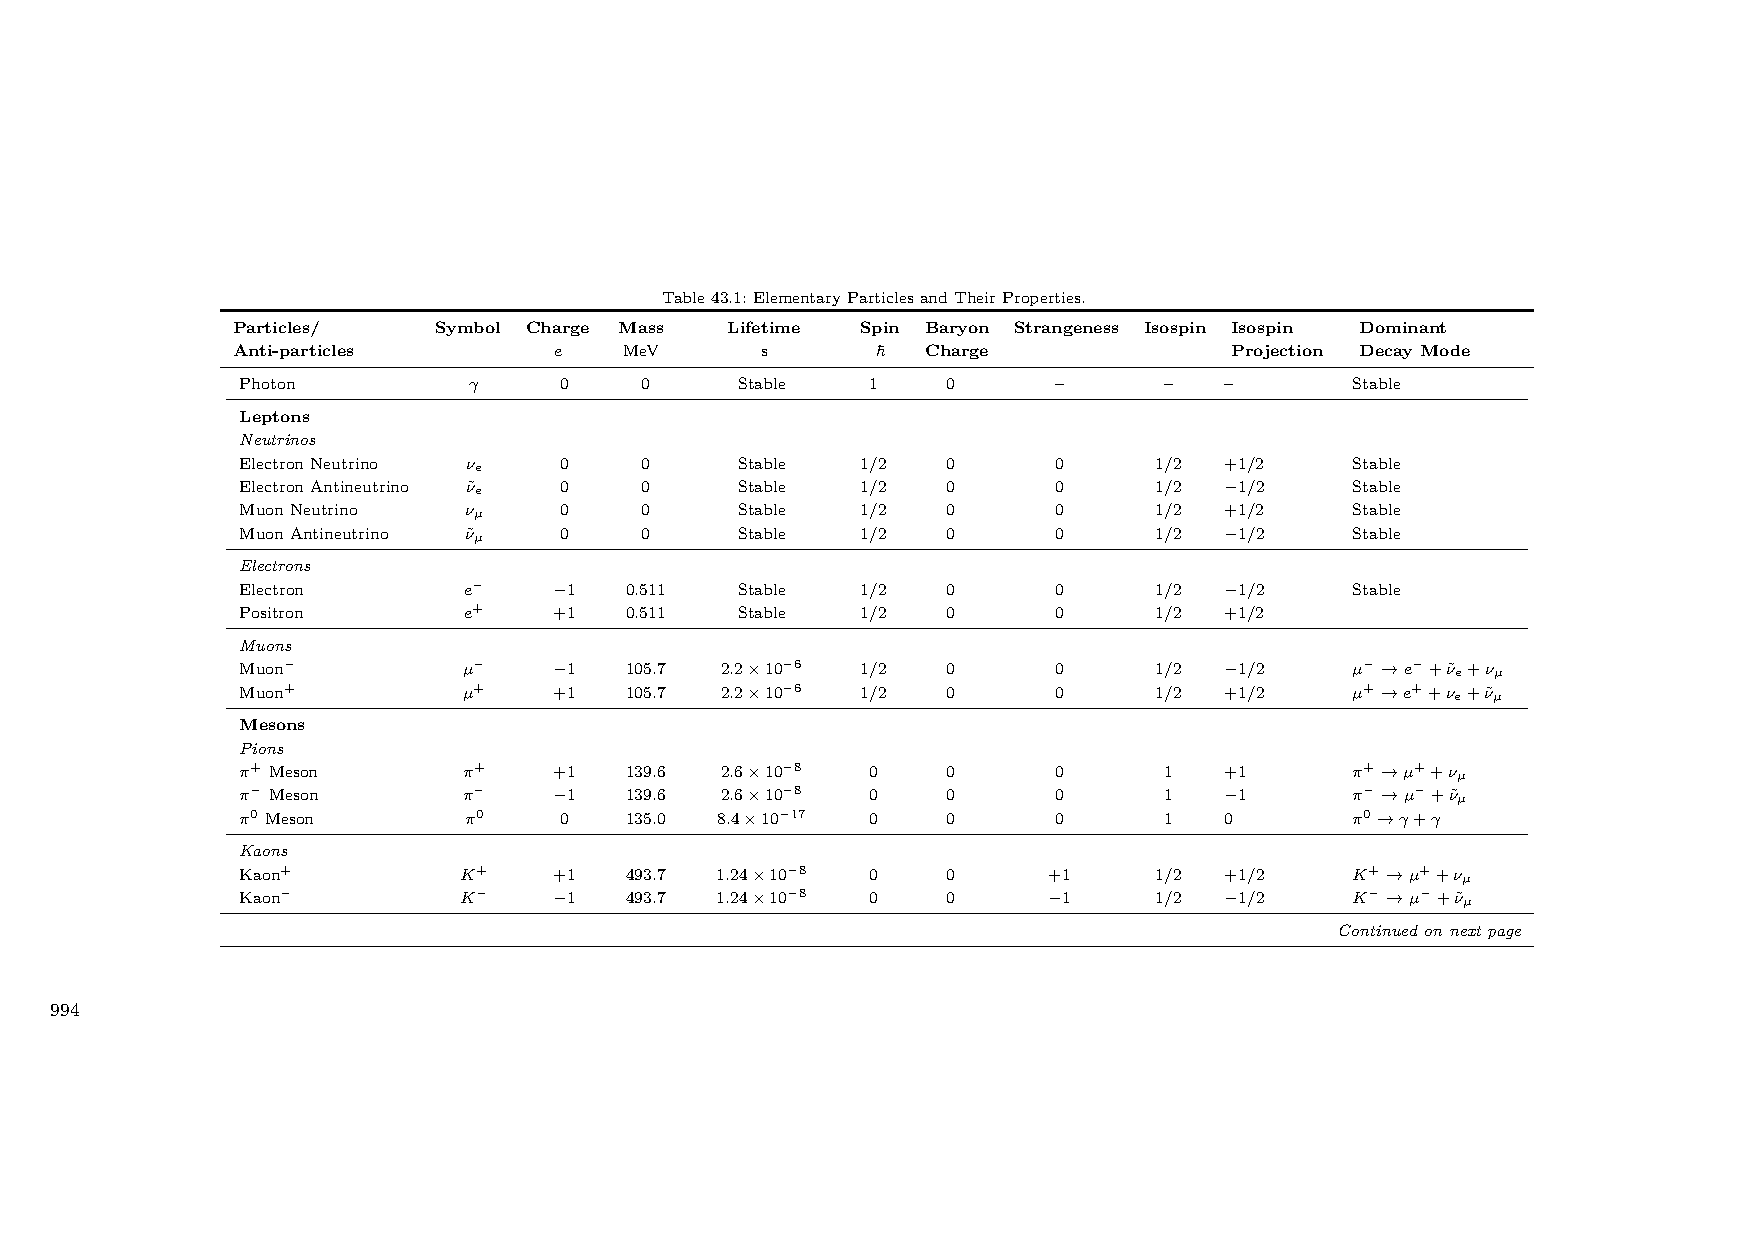
\includepdf[pages=-,scale=1.3]{figs/ch-43/elemparttables.pdf}
\setcounter{page}{997}

\subsection{}\label{43.1.2} In energy regions less than $2m_{0}c^{2}$ (where $m_{0}$ is the rest mass of the particle), the structure of particles has no effect on interaction between them and other particles and fields. In
these cases elementary particles are dealt with as particles in the sense of material points, but possessing many properties, such as: rest mass, electric charge, spin and a dominant decay mode (\tabl{tab-43.1}). The concept of a point elementary particle meets the requirements of relativity theory. An extended particle of finite dimensions, which is an integral whole, should not be deformable as otherwise independent movements of its parts would be possible. But this would mean that external action on such an elementary particle would be instantaneously transmitted from certain parts to others, and this contradicts relativity theory \ssect{5.1.1}.
\zhpar{在能量小于 $2m_{0}c^{2}$（其中 $m_{0}$ 为粒子的静止质量）的能区中，粒子的结构对它与其他粒子及场的相互作用没有影响。在这种情况下，基本粒子可以当作质点来处理，但它具有许多性质，例如静止质量、电荷、自旋以及主要衰变方式（见\tabl{tab-43.1}）。点状基本粒子的概念符合相对论的要求。有限大小的扩展粒子是一个整体，它不应当是可形变的，否则其各部分就可能有独立的运动。但这意味着对该基本粒子的外部作用将从某些部分瞬时传递到其他部分，这与相对论相矛盾（参见\ssect{5.1.1}）。}

\subsection{}\label{43.1.3}. A structureless charged elementary particle has an infinite potential \ssect{16.2.6} and infinite potential energy. Up-to-date particle physicists are working out various methods of introducing nonpoint-like interaction. These methods eliminate the ``infinity'' of point elementary particles, and introduce definite structures for them without contradicting relativity theory.
\zhpar{没有结构的带电基本粒子具有无穷大的电势（参见\ssect{16.2.6}）和无穷大的势能。当前的粒子物理学家正在研究引入非点状相互作用的各种方法。这些方法可以消除点状基本粒子的“无穷大”，并在不违背相对论的前提下为其引入确定的结构。}

It follows from the indeterminacy relations \ssect{38.6.2} that a study of the structure of elementary particles requires the investigation of processes taking place at the extremely short distances $\delta$ that the momentum indeterminacy $\Delta p \geqslant \hbar/ \delta$ corresponds
to. The shorter the distances $\delta$ , associated with the structure of elementary particles, the greater the momentum $p$ of the particles must be, because it cannot be less than $\Delta p$. Consequently, the structure of elementary particles can be cleared up only by research involving high energies. For this reason, particle physics, the new branch of physics engaged in the study of elementary particles, is now more commonly called \redem{high-energy physics}.
\zhpar{由不确定关系（\ssect{38.6.2}）可知，研究基本粒子的结构需要考察极短距离 $\delta$ 上发生的过程，该距离所对应的动量不确定量满足 $\Delta p \geqslant \hbar/ \delta$。与基本粒子结构相关的距离 $\delta$ 越短，粒子的动量 $p$ 就必须越大，因为它不可能小于 $\Delta p$。因此，只有借助高能研究，才能弄清基本粒子的结构。正因为如此，专门研究基本粒子的物理学新分支——粒子物理学，现在更多地被称为\redem{高能物理学}。}

\section{Classification of Elementary Particles and Their
Interaction}
\label{sec-43.2} 
\zhtitle{基本粒子的分类及其相互作用}


\subsection{}\label{43.2.1} There are several groups of elementary particles which differ in their properties and the nature of the interaction between one another.
\zhpar{基本粒子有若干类，它们的性质以及彼此之间相互作用的性质各不相同。}

The main classification of elementary particles is based on their various rest masses: distinction is made between \redem{leptons} (light particles), \redem{mesons} (intermediate particles) and \redem{baryons} (heavy particles), with the last being further subdivided into \redem{nucleons} and \redem{hyperons}.
\zhpar{基本粒子的主要分类依据是其静止质量的不同：可分为\redem{轻子}（轻粒子）、\redem{介子}（中等质量粒子）和\redem{重子}（重粒子），其中重子又进一步分为\redem{核子}和\redem{超子}。}

\subsection{}\label{43.2.2} As to their electric charge, measured in units of the elementary charge $e$ \ssect{14.1.2}, particles may be positive, negative
or neutral. The existence of particles with fractional electric charges, called \redem{quarks}, has been predicted.
With respect to their spin \ssect{26.1.3}, elementary particles are subdivided into ones with integer, half-integer and zero spin (in units of h). Depending upon their spin, assemblies of particles comply with different quantum statistics \ssect{41.2.1} and \ssect{41.2.4}.
\zhpar{就电荷而言，以基本电荷 $e$（参见\ssect{14.1.2}）为单位度量时，粒子可以带正电、带负电或不带电。人们已预言存在电荷为分数的粒子，称为\redem{夸克}。就自旋而言（参见\ssect{26.1.3}），基本粒子可分为自旋为整数、半整数和零的粒子（以 h 为单位）。根据自旋的不同，粒子体系遵从不同的量子统计（参见\ssect{41.2.1}和\ssect{41.2.4}）。}

\subsection{}\label{43.2.3} Elementary particles are either \redem{stable} or \redem{unstable}. This classification characterizes their lifetime and the dominant decay mode. The characteristics of elementary particles are listed in \tabl{tab-43.1}. The rest masses of the particles are given in energy units, as is now customary practice, on the basis of the relation $E = mc_{2}$ \ssect{5.7.2}. Since the rest mass of the electron is approximately \SI{0.5}{MeV}, the mass of a particle in electron mass units can be found by multiplying its mass in \si{\MeV} by two.
\zhpar{基本粒子或是稳定的，或是不稳定的。这种分类反映了粒子的寿命和主要衰变方式。基本粒子的特性列于\tabl{tab-43.1}中。按照现在通行的做法，粒子的静止质量以能量单位给出，其依据是关系式 $E = mc_{2}$（参见\ssect{5.7.2}）。由于电子的静止质量约为\SI{0.5}{MeV}，因此以电子质量为单位表示的粒子质量，可以将其以\si{\MeV}为单位的质量乘以二求得。}

\subsection{}\label{43.2.4} In addition to the elementary particles listed in \tabl{tab-43.1}, there are also a great many particles called \redem{resonances}
(\redem{resonons} and \redem{resonance particles}). Their lifetimes are characteristic of strong interaction \ssect{43.2.5}; they have definite properties, energies and momenta, and definite decay modes. These features enable resonances to be regarded as special particles.
\zhpar{除\tabl{tab-43.1}所列的基本粒子外，还有大量被称为\redem{共振态}（\redem{共振子}和\redem{共振粒子}）的粒子。它们的寿命具有强相互作用的特征（参见\ssect{43.2.5}）；它们具有确定的性质、能量和动量，以及确定的衰变方式。这些特征使共振态可以被视为特殊的粒子。}

\subsection{}\label{43.2.5} Mainly three of the four known kinds of interaction exist between elementary particles: strong, electromagnetic and weak. Gravitational interaction between elementary particles is usually not considered. Each of the interactions is characterized by its \redem{interaction coupling constant}, determining its comparative magnitude, and its characteristic interaction time (\redem{time constant of interaction}).
\zhpar{基本粒子之间主要存在四种已知相互作用中的三种：强相互作用、电磁相互作用和弱相互作用。通常不考虑基本粒子之间的引力相互作用。每一种相互作用都由其\redem{相互作用耦合常量}来表征，该常量决定其相对强弱；每一种相互作用还有其特征作用时间（\redem{相互作用的时间常数}）。}

\subsection{}\label{43.2.6} \redem{Strong interactions} refer to processes involving baryons, as well as pions and kaons (\tabl{tab-43.1}). Strong interactions result from nuclear forces between nucleons \ssect{42.3.1}, as well as the processes of creation and decay of mesons and hyperons in nuclear reactions at high energies. Strong interaction is characterized by the \redem{Fermi constant} $\beta = f^{2}/\hbar c \approx 1$, where the constant $f$ has the dimension of an electric charge. Processes that display strong interaction are said to be fast and have a characteristic
\redem{nuclear time} $\tau_{N}$. In order of magnitude this time equals the Compton wavelength of the nucleon $h/m_{p} c$ (where $m_{p}$ is the mass of the nucleon), divided by the velocity of light in free space, i.e. $h/m_{p} c^{2}$.
Particles that take part in strong interactions are called \redem{hadrons} (large and heavy particles).
\zhpar{\redem{强相互作用}涉及重子以及π介子和K介子（见\tabl{tab-43.1}）的过程。强相互作用源于核子之间的核力（参见\ssect{42.3.1}），也源于高能核反应中介子和超子的产生与衰变过程。强相互作用由\redem{费米常量} $\beta = f^{2}/\hbar c \approx 1$ 来表征，其中常量 $f$ 具有电荷的量纲。表现出强相互作用的过程称为快过程，其特征时间为\redem{核时间} $\tau_{N}$。在数量级上，该时间等于核子的康普顿波长 $h/m_{p} c$（其中 $m_{p}$ 为核子的质量）除以真空中的光速，即 $h/m_{p} c^{2}$。参与强相互作用的粒子称为\redem{强子}（大而重的粒子）。}

\subsection{}\label{43.2.7} \redem{Electromagnetic interactions} characterize processes that take place between particles that have electric charges. For instance, Coulomb repulsion in nuclei, and the processes of creation and annihilation of electron-positron pairs are associated with electromagnetic interaction. A measure of this interaction is a dimensionless constant called the \redem{fine-structure
constant}: $\alpha = e^{2}/\hbar c = 1/137$. It has been thus named because a determines the magnitude of fine splitting of the atom's energy level into a number of sublevels. This is caused by the effect of the relativistic dependence of mass on velocity \ssect{5.6.1} on
the electron's energy in the atom. 
\zhpar{\redem{电磁相互作用}表征带电粒子之间发生的过程。例如，原子核中的库仑斥力，以及电子-正电子对的产生与湮灭过程，都与电磁相互作用有关。这种相互作用的度量是一个无量纲常量，称为\redem{精细结构常量}：$\alpha = e^{2}/\hbar c = 1/137$。之所以如此命名，是因为 $\alpha$ 决定了原子能级精细分裂为若干子能级的大小。这种精细分裂是由于原子中电子的能量受到质量随速度变化这一相对论效应的影响（参见\ssect{5.6.1}）而产生的。}

Processes accompanying electromagnetic interaction are called electromagnetic processes and they proceed during a time of the order of \SIrange{d-20}{d-18}{\second} in accordance with the fact that $\alpha/\beta \approx \num{d-2}$ \ssect{43.2.6}. Electromagnetic interaction is the only one of the interactions of the microcosm that is also manifested in macroscopic phenomena and processes.
\zhpar{伴随电磁相互作用的过程称为电磁过程，其持续时间的数量级为 \SIrange{d-20}{d-18}{\second}，这与 $\alpha/\beta \approx \num{d-2}$ 的事实相一致（参见\ssect{43.2.6}）。在微观世界的各种相互作用中，电磁相互作用是唯一同时表现于宏观现象和过程中的相互作用。}

\begin{small}
\begin{table}
\begin{center}
\begin{tabular}{p{2.5cm}p{2cm}p{2.5cm}}
\toprule
\textbf{Interaction} & \textbf{Relative Strength} & \textbf{Interaction Time} s\\
\midrule
Strong & 1 & \numrange{d-23}{d-22} \\
Electromagnetic & 1/137 & \numrange{d-20}{d-18} \\
Weak & \num{d-14} & \numrange{d-10}{d-8} \\
\bottomrule
\end{tabular}
\end{center}
\sidecaption{Properties of interaction forces in elementary particles.\zhcap{基本粒子中相互作用力的性质。} \label{tab-43.2}}
\end{table}
\end{small}

\subsection{}\label{43.2.8} \redem{Weak interactions} are processes involving leptons (\tabl{tab-43.1}). Examples of such processes are beta decay of nuclei \ssect{42.6.1}, and interaction between nuclei and muons, electrons (or positrons), and neutrinos (or antineutrinos).
\zhpar{\redem{弱相互作用}是涉及轻子的过程（见\tabl{tab-43.1}）。例如原子核的β衰变（参见\ssect{42.6.1}），以及原子核与μ子、电子（或正电子）和中微子（或反中微子）之间的相互作用，都属于这类过程。}

Weak interaction is characterized by the \redem{weak interaction constant} $G$, having the dimension of the inverse square of mass. The dimensionless weak interaction constant $g^{2} = Gm_{p}^{2} \approx \num{d-5}$, where $m_{p}$ is the mass of the proton. Weak interaction is the
slowest of the interactions manifested in the microcosm and
proceeds during time of the order of \SI{d-10}{\second}. A comparison of the various kinds of interaction between elementary particles is given in \tabl{tab-43.2}.
\zhpar{弱相互作用由\redem{弱相互作用常量} $G$ 来表征，它的量纲为质量平方的倒数。无量纲的弱相互作用常量为 $g^{2} = Gm_{p}^{2} \approx \num{d-5}$，其中 $m_{p}$ 为质子的质量。弱相互作用是微观世界中所有相互作用里最慢的一种，其过程持续时间的数量级为 \SI{d-10}{\second}。各种基本粒子相互作用的比较列于\tabl{tab-43.2}中。}

\section{Certain Information on Various Elementary Particles}
\label{sec-43.3} 


\subsection{}\label{43.3.1} Various kinds of elementary particles (\tabl{tab-43.1}) are produced in the interaction of cosmic rays with the nuclei of the nitrogen and oxygen atoms in the atmosphere. Since the development of modern accelerators, the creation, mutual transformations and structure of elementary particles are investigated in the laboratory.
\zhpar{各种基本粒子（见\tabl{tab-43.1}）是宇宙射线与大气中氮原子和氧原子的原子核相互作用时产生的。自现代加速器发展以来，人们便在实验室中研究基本粒子的产生、相互转化及其结构。}

\subsection{}\label{43.3.2} The feasibility of creating new particles in the interaction between protons and nuclei follows from the relation between mass and energy \ssect{5.7.2}. When an energy of \SI{d4}{\GeV} is imparted
to the proton, approximately \num{d4} times more than its rest energy $m_{p}c^{2}$ (where $m_{p}$ is the rest mass of the proton and $c$ is the velocity of light in free space), a collision between the proton and a nucleus leads to splitting of the latter. High kinetic energy is imparted to the fission products and new particles are created, some having a rest mass and others without one.
\zhpar{质子与原子核相互作用时产生新粒子的可能性，可由质量与能量的关系（参见\ssect{5.7.2}）得出。当质子获得 \SI{d4}{\GeV} 的能量时（约为其静止能量 $m_{p}c^{2}$ 的 \num{d4} 倍，其中 $m_{p}$ 为质子的静止质量，$c$ 为真空中的光速），质子与原子核的碰撞将导致后者发生分裂。分裂产物获得很大的动能，并产生新的粒子，其中一些具有静止质量，另一些则没有。}

\subsection{}\label{43.3.3} \redem{Muons (mu mesons)} are the electrically charged particles $\mu_{+}$ and $\mu_{-}$ with a rest mass equal approximately to $200~m_{e}$, where $m_{e}$ is the rest mass of the electron. The main characteristics of muons are listed in \tabl{tab-43.1}. Muons are not stable, and decay according to the modes:
\zhpar{\redem{μ子}（即μ介子）是带电粒子 $\mu_{+}$ 和 $\mu_{-}$，其静止质量约为 $200~m_{e}$，其中 $m_{e}$ 为电子的静止质量。μ子的主要特性列于\tabl{tab-43.1}中。μ子是不稳定的，按以下方式衰变：}
\begin{align*}%
\mu^{+} & \to \ce{^{0}_{+1}e} + \ce{^{0}_{0}{\nu_{e}}} + \ce{^{0}_{0}{\tilde{\nu}_{\mu}}} \qand \\
\mu^{-} & \to \ce{^{0}_{-1}e} + \ce{^{0}_{0}{\tilde{\nu}_{e}}} + \ce{^{0}_{0}{\nu_{\mu}}}
\end{align*}
where \ce{^{0}_{-1}e} and \ce{^{0}_{+1}e} are the electron and positron, $\ce{^{0}_{0}\nu_{e}}$ and $\ce{^{0}_{0}\tilde{\nu_{e}}}$ are the electron neutrino and antineutrino, $\ce{^{0}_{0}\nu_{\mu}}$ and $\ce{^{0}_{0}\tilde{\nu_{\mu}}}$ are the muon neutrino and antineutrino.
\zhpar{式中 \ce{^{0}_{-1}e} 和 \ce{^{0}_{+1}e} 分别为电子和正电子，$\ce{^{0}_{0}\nu_{e}}$ 和 $\ce{^{0}_{0}\tilde{\nu_{e}}}$ 分别为电子中微子和反中微子，$\ce{^{0}_{0}\nu_{\mu}}$ 和 $\ce{^{0}_{0}\tilde{\nu_{\mu}}}$ 分别为μ中微子和反中微子。}

The \redem{muon neutrino} (or \redem{antineutrino}) is a particle having neither rest mass nor electric charge, and which is emitted in the creation and decay of mesons. These particles differ from the neutrino (or anti-neutrino) emitted together with electrons in beta-decay processes \ssect{42.6.1}. Therefore, the two types of neutrino (and antineutrino) are designated by different symbols:
$\ce{^{0}_{0}\nu_{e}}, \; \ce{^{0}_{0}\tilde{\nu_{e}}}$
and $\ce{^{0}_{0}\nu_{\mu}} \; \ce{^{0}_{0}\tilde{\nu_{\mu}}}$. The spin of the mu mesons equals $\pm \hbar /2$ and the muon decay reaction complies with the conservation laws \ssect{42.9.2}. The interaction of muons with nuclei is an example of weak interaction \ssect{43.2.8}, and muons are nuclearly inactive particles.
\zhpar{\redem{μ中微子}（或\redem{反中微子}）是既没有静止质量也不带电荷的粒子，它在介子的产生和衰变过程中被放出。这些粒子不同于在β衰变过程中与电子一同放出的中微子（或反中微子）（参见\ssect{42.6.1}）。因此，两种中微子（及反中微子）用不同的符号表示，即 $\ce{^{0}_{0}\nu_{e}}, \; \ce{^{0}_{0}\tilde{\nu_{e}}}$ 与 $\ce{^{0}_{0}\nu_{\mu}} \; \ce{^{0}_{0}\tilde{\nu_{\mu}}}$。μ子的自旋等于 $\pm \hbar /2$，μ子的衰变反应符合守恒定律（参见\ssect{42.9.2}）。μ子与原子核的相互作用是弱相互作用的一个例子（参见\ssect{43.2.8}），μ子是不参与核相互作用的粒子。}

\subsection{}\label{43.3.4} \redem{Pions (pi mesons)} are neutral ($\pi^{0}$) and electrically charged ($\pi^{+}$ and $\pi^{-}$) particles with a rest mass of approximately $300~m_{e}$, where me is the rest mass of the electron. The main characteristics of pions are listed in \tabl{tab-43.1}. Pions, like muons, are unstable and decay according to the modes:
\zhpar{\redem{π介子}（又称 pi 介子）是中性粒子（$\pi^{0}$）和带电粒子（$\pi^{+}$ 和 $\pi^{-}$），其静止质量约为 $300~m_{e}$，其中 $m_{e}$ 为电子的静止质量。π介子的主要特性列于\tabl{tab-43.1}中。π介子与μ子一样是不稳定的，按以下方式衰变：}
\begin{align*}%
\pi^{+} & \to \mu^{+} + \ce{^{0}_{0}\nu_{\mu}},\\
\pi^{-} & \to \mu^{-} + \ce{^{0}_{0}\tilde{\nu_{\mu}}}, \qand \\
\pi^{0} & \to \gamma + \gamma.
\end{align*}
In these decay reactions $\mu^{+}$ and $\mu^{-}$ are the positive and negative muons, respectively. $\ce{^{0}_{0}{\nu_{\mu}}}$ and $\ce{^{0}_{0}{\tilde{\nu}_{\mu}}}$ are the muon neutrino and antineutrino, and $\gamma$ is a gamma-ray quantum (photon). Shown schematically in \figr{fig-43-01} is the sequence for the ($\pi$-$\mu$-$e$) decays. Pions are spinless particles. This follows from their decay reactions and the requirement that these reactions comply with the conservation laws.
\zhpar{式中 $\mu^{+}$ 和 $\mu^{-}$ 分别为正μ子和负μ子；$\ce{^{0}_{0}{\nu_{\mu}}}$ 和 $\ce{^{0}_{0}{\tilde{\nu}_{\mu}}}$ 分别为μ中微子和反中微子，$\gamma$ 为γ射线量子（光子）。（$\pi$-$\mu$-$e$）衰变的顺序示意图见\figr{fig-43-01}。π介子是自旋为零的粒子，这由其衰变反应以及这些反应需符合守恒定律的要求得出。}
\begin{marginfigure}%[-2cm] 
\centering
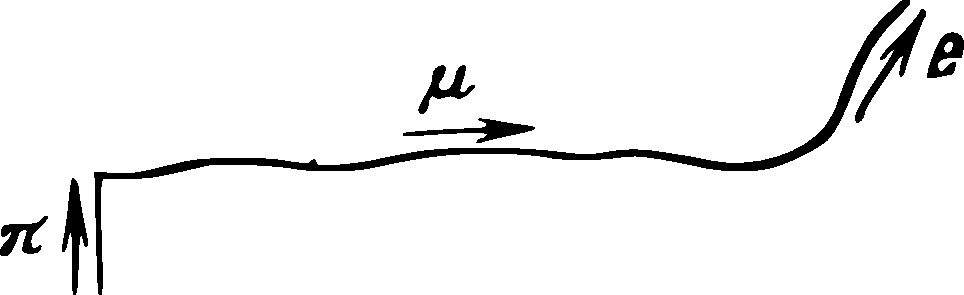
\includegraphics[width=\textwidth]{figs/ch-43/fig-43-01.pdf}
\sidecaption{Schematic visualisation of $\pi$-$\mu$-$e$ decays.\label{fig-43-01}}
\end{marginfigure}

\subsection{}\label{43.3.5} Pions are formed in cosmic rays as the result of the disintegration of the nuclei of atmospheric gas atoms by fast protons and alpha particles. To produce pions the energy of the protons should be about \SI{300}{\MeV}.
\zhpar{π介子是宇宙射线中由快速质子和α粒子使大气中气体原子的原子核发生分裂而产生的。要产生π介子，质子的能量应约为 \SI{300}{\MeV}。}

The arrangement for obtaining pions in the laboratory is illustrated in \figr{fig-43-02}. Target $A$ of beryllium or carbon is bombarded by fast protons \ce{^{1}_{1}p}. This knocks pions out of the target at arbitrary angles. The magnetic field of the accelerator causes the ejected pions to follow circular paths whose radii are determined by the velocities of the pions. Pions ejected in the forward direction are divided into two beams, the negative ones being deflected outside the accelerator chamber and the positive ones inside. The opposite is true for pions ejected in the backward direction (not shown in \figr{fig-43-02}).
\zhpar{在实验室中获得π介子的装置如\figr{fig-43-02}所示。靶 $A$ 由铍或碳制成，被快速质子 \ce{^{1}_{1}p} 轰击，从而使靶中以任意角度射出π介子。加速器的磁场使射出的π介子沿圆轨道运动，其轨道半径由π介子的速度决定。沿前进方向射出的π介子分为两束：带负电的π介子在加速器真空室外偏转，带正电的π介子则在室内偏转。对于沿后方射出的π介子，情况正好相反（未在\figr{fig-43-02}中画出）。}

\begin{marginfigure}%[-2cm] 
\centering
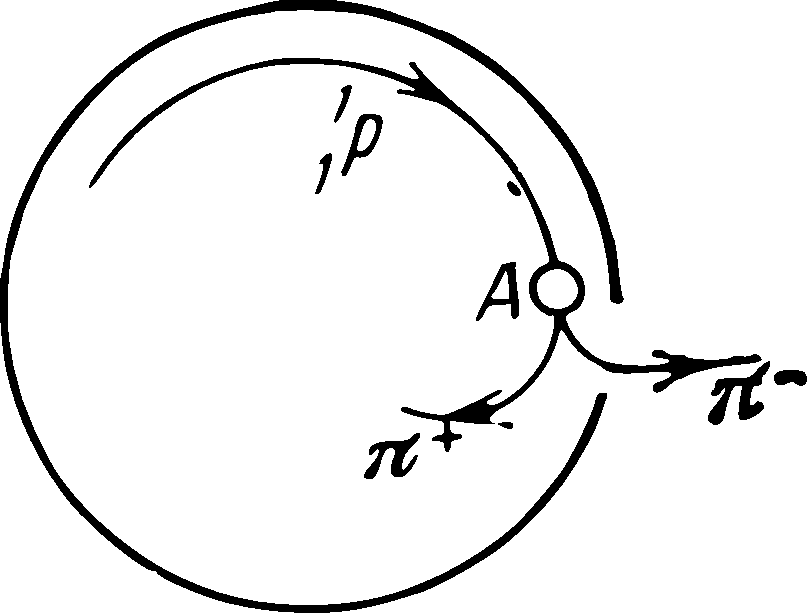
\includegraphics[width=\textwidth]{figs/ch-43/fig-43-02.pdf}
\sidecaption{Schematic arrangement for obtaining pions in the laboratory.\zhcap{实验室中获得π介子的示意装置。}\label{fig-43-02}}
\end{marginfigure}


The masses of charged ions are determined by their energies
and momenta by methods employing the deflection of particles
in magnetic and electric fields. The lifetime of pions (\tabl{tab-43.1}) is established by measuring the time intervals between the instant of creation of a pion and its instant of decay \ssect{43.3.4}. Pions are nuclearly active particles. Their interaction with nuclei is an example of strong interaction \ssect{43.2.6}.
\zhpar{带电粒子的质量由其能量和动量确定，测定方法利用粒子在磁场和电场中的偏转。π介子的寿命（见\tabl{tab-43.1}）是通过测量π介子产生时刻与衰变时刻之间的时间间隔而确定的（参见\ssect{43.3.4}）。π介子是具有核活性的粒子，它与原子核的相互作用是强相互作用的一个例子（参见\ssect{43.2.6}）。}

Similar methods are applied for investigating other charged
particles. Since neutral particles are not deflected in a magnetic field, they arc investigated by means of the conservation laws and interaction reactions of the given particle with other particles. For example, the reaction of a negative pion with a proton proceeds according to the mode
\zhpar{对其他带电粒子也可以采用类似的方法进行研究。由于中性粒子在磁场中不发生偏转，因此只能借助守恒定律以及该粒子与其他粒子的相互作用反应来研究它们。例如，负π介子与质子的反应按以下方式进行：}
\begin{equation*}%
\pi^{+} + \ce{^{1}_{1}p} \to \pi^{0} + \ce{^{1}_{0}n}.
\end{equation*}
The negative pion is transformed into a neutral one, and the
proton into a neutron. The neutral pion $\pi^{0}$ decays into two gamma-ray quanta \ssect{43.3.4}. The mass of the neutral pion (\tabl{tab-43.1}) is determined from the known masses and energies of the proton, neutron and negative pion, from the energy of gamma-ray quanta, as well as from data on the momenta of particles in these transformations.
\zhpar{负π介子转变为中性π介子，质子转变为中子。中性π介子衰变为两个γ射线量子（参见\ssect{43.3.4}）。中性π介子的质量（见\tabl{tab-43.1}）是根据质子、中子和负π介子的已知质量与能量、γ射线量子的能量，以及这些转变过程中粒子动量的数据确定的。}

\subsection{}\label{43.3.6} The principle of applying the law of conservation of momentum for studying the transformations of elementary particles can be illustrated by the example of the $\beta^{-}$ decay in which an electron antineutrino $\ce{^{0}_{0}\tilde{\nu_{e}}}$  created \ssect{42.6.1}. If only a single electron were ejected by the nucleus in a $\beta^{-}$ decay, the nucleus would be subject to recoil in the direction directly opposite to that of the ejected electron. The momentum of the nucleus that was stationary before the decay reaction would be equal in magnitude but opposite in direction to that of the ejected electron. If, however, in addition to the electron, the nucleus also ejects an antineutrino, the vector sum of the three momenta. that of the electron, antineutrino and recoil nucleus, should, according to the law of conservation of momentum \ssect{2.7.1}, be equal to zero, as before the decay reaction (\figr{fig-43-03}).
\zhpar{利用动量守恒定律研究基本粒子的转变，可以用 $\beta^{-}$ 衰变中产生电子反中微子 $\ce{^{0}_{0}\tilde{\nu_{e}}}$ 的过程来说明（参见\ssect{42.6.1}）。若在 $\beta^{-}$ 衰变中原子核只放出一个电子，则原子核将沿与电子运动方向正好相反的方向反冲。衰变前静止的原子核，其动量的大小与射出电子的动量相等，方向则相反。然而，若原子核除放出电子外还放出一个反中微子，那么根据动量守恒定律（参见\ssect{2.7.1}），电子、反中微子和反冲核三者动量的矢量和应当为零，与衰变反应前相同（见\figr{fig-43-03}）。}

\begin{marginfigure}[-3cm] 
\centering
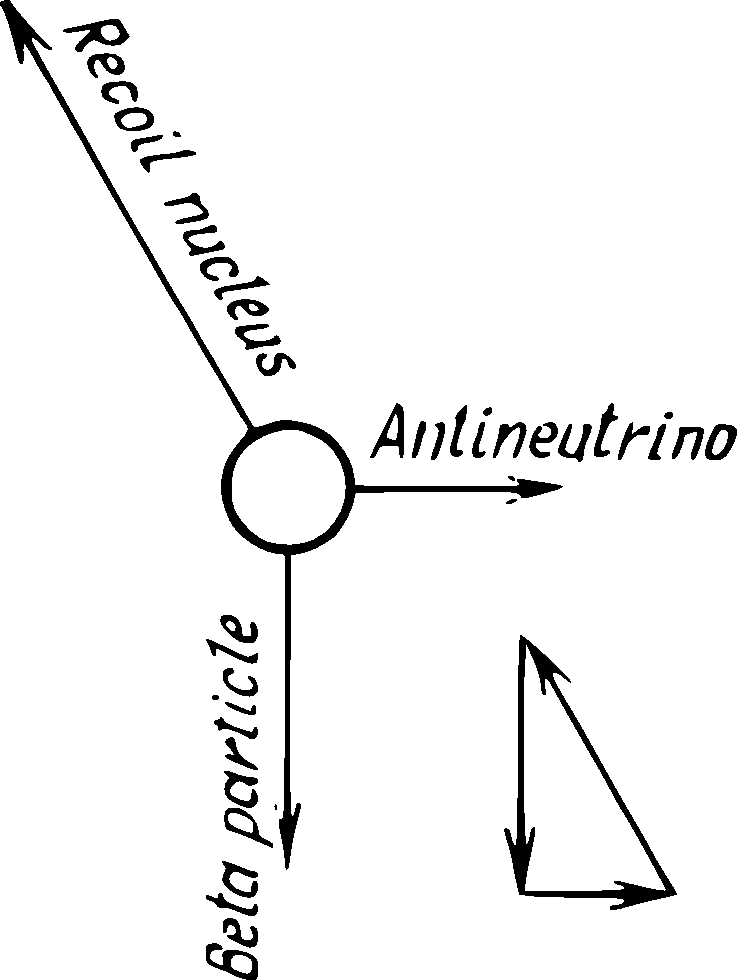
\includegraphics[width=0.7\textwidth]{figs/ch-43/fig-43-03.pdf}
\sidecaption{Schematic illustration of $\beta^{-}$ decay according to the law of conservation of momentum.\zhcap{依据动量守恒定律的 $\beta^{-}$ 衰变示意图。}\label{fig-43-03}}
\end{marginfigure}


\subsection{}\label{43.3.7} \redem{Kaons}, or \redem{$K$ mesons}, are neutral ($K^{0}$) and charged ($K^{+}$ and $K^{-}$) particles with rest masses close to $1000~m_{e}$, where $m_{e}$ is the rest mass of the electron. As other mesons, kaons are unstable, but, in contrast to the decay reactions of pions and muons (\ssect{43.3.3} and \ssect{43.3.4}), the reaction channels of their decays are not unambiguous. As a result of kaon decay, pions, muons and neutrinos (or antineutrino) of both types are formed. Like pions, kaons are spinless. All of these particles (pions and kaons) are united in a single group, the mesons (\tabl{tab-43.1}).
\zhpar{\redem{K介子}是中性粒子（$K^{0}$）和带电粒子（$K^{+}$ 和 $K^{-}$），其静止质量接近 $1000~m_{e}$，其中 $m_{e}$ 为电子的静止质量。与其他介子一样，K介子是不稳定的。但与π介子和μ子的衰变反应（参见\ssect{43.3.3}和\ssect{43.3.4}）不同，K介子的衰变道并不是唯一确定的。K介子衰变的结果会产生π介子、μ子以及两种类型的中微子（或反中微子）。与π介子一样，K介子是自旋为零的粒子。所有这些粒子（π介子和K介子）同属于一个类别，即介子（见\tabl{tab-43.1}）。}

\subsection{}\label{43.3.8} A large group of particles called \redem{hyperons}, have rest masses greater than that of nucleons, and range approximately from $2183~m_{e}$ for the lambda-zero hyperon ($\Lambda^{0}$) to $3280~m_{e}$ for the omega-minus hyperon ($\Omega^{-}$). Hyperons are unstable (see \tabl{tab-43.1}). The lighter hyperons decay into nucleons and pions.
\zhpar{有一大类称为\redem{超子}的粒子，其静止质量大于核子，范围大致从 $\Lambda^{0}$ 超子（$2183~m_{e}$）到 $\Omega^{-}$ 超子（$3280~m_{e}$）。超子是不稳定的（见\tabl{tab-43.1}）。较轻的超子衰变为核子和π介子。}

The heavier hyperons decay into lighter hyperons, pions and
kaons. All hyperons have a spin equal to $\hbar / 2$, except the $\Omega^{-}$ hyperon, whose spin is equal to $3\hbar /2$. Nucleons (protons and neutrons) and hyperons are related particles and they belong to a single class of heavy particles called baryons (\tabl{tab-43.1}).
\zhpar{较重的超子衰变为较轻的超子、π介子和K介子。除 $\Omega^{-}$ 超子的自旋等于 $3\hbar /2$ 外，所有超子的自旋均等于 $\hbar / 2$。核子（质子和中子）与超子是相关的粒子，它们同属于一类重粒子，称为\redem{重子}（见\tabl{tab-43.1}）。}

\section[Conservation Laws of Elementary Particles]{Certain Conservation Laws in Elementary-Particle Physics}
\label{sec-43.4} 
\zhtitle{基本粒子物理学中的某些守恒定律}

\subsection{}\label{43.4.1} The differences in the rest masses of charged $\pi^{\pm}$ and the neutral $\pi^{0}$ pions, like the difference in the rest masses of the
two stales of nucleons-proton and neutron-in the nucleus,
are the result of charge independence of nuclear forces \ssect{42.3.3} and of the presence of electromagnetic interactions in addition to strong nuclear interactions. With no electromagnetic interactions in the nucleus, charge independence of nuclear forces would lead to a condition in which the proton and neutron have equal rest mass, and the masses of all types of pions coincide.
\zhpar{带电的 $\pi^{\pm}$ 介子与中性的 $\pi^{0}$ 介子在静止质量上的差异，以及原子核中两种核子态（质子和中子）静止质量上的差异，都是由核力的电荷无关性（参见\ssect{42.3.3}）以及除强核相互作用外还存在电磁相互作用所引起的。若原子核中不存在电磁相互作用，核力的电荷无关性将导致质子与中子的静止质量相等，所有类型的π介子的质量也都相同。}

When the additional electromagnetic interaction is taken into account, the double state of the nucleon (\redem{proton-neutron doublet}) is split into two different states in accordance with their rest masses. The masses of the neutron and proton are found to differ. For the same reason, the masses of the particles that make up the \redem{pion triplet} are also not equal to one another. The masses of the charged $\pi^{\pm}$ pions exceed that of the $\pi^{0}$ pion (\tabl{tab-43.1}).
\zhpar{在考虑附加的电磁相互作用后，核子的双重态（\redem{质子-中子二重态}）按静止质量的不同分裂为两种不同的状态。中子与质子的质量被发现存在差异。出于同样的原因，组成\redem{π介子三重态}的粒子，其质量彼此也不相等。带电的 $\pi^{\pm}$ 介子的质量超过 $\pi^{0}$ 介子的质量（见\tabl{tab-43.1}）。}

\subsection{}\label{43.4.2} Introduced to characterize the multiplicity of states of certain kinds of particles are the concepts of \redem{isotopic spin} $T$ (\redem{isospin}) and the \redem{projection $T_{\xi}$ of isotopic spin} on a certain ``axis''. The introduction of these characteristics of elementary particles makes it possible to formulate special features of the properties and transformation of elementary particles that follow from charge independence in strong interactions. Isotopic spin $T$ characterizes the number of particles in the given ``charge multiplet''; this number is equal to $(2T + 1)$. Thus the isotopic spin of the nucleon equals $T = 1/2$, and that of the pion is $T = 1$, in accordance with the number of particles (nucleons and pions) in the doublet and triplet.
\zhpar{为表征某些粒子的多重态，引入了\redem{同位旋}（isotopic spin）$T$（又称 isospin），以及在某一“轴”上的\redem{同位旋投影} $T_{\xi}$ 的概念。引入这些基本粒子的特征量，使人们可以阐明由强相互作用中电荷无关性所决定的基本粒子性质及其转变的特殊规律。同位旋 $T$ 表征给定“电荷多重态”中粒子的数目，该数目等于 $(2T + 1)$。因此，核子的同位旋 $T = 1/2$，π介子的同位旋 $T = 1$，这与双重态（核子）和三重态（π介子）中的粒子数目相对应。}

The projection $T_{\xi}$ of isotopic spin of the nucleon is introduced in such a way that it is related to the charge $Z$ (in $e$ units) of a particle that is a member of a charge doublet as follows:
\zhpar{核子同位旋投影 $T_{\xi}$ 的引入方式，使其与属于电荷双重态的粒子所带电荷 $Z$（以 $e$ 为单位）之间满足如下式所示的关系。}
\begin{equation*}%
Z = T_{\xi} + \frac{1}{2}.
\end{equation*}
For the neutron $T_{\xi} = -1/2$, for the proton $T_{\xi} = +1/2$.
\zhpar{对于中子，$T_{\xi} = -1/2$；对于质子，$T_{\xi} = +1/2$。}

For the triplet of pions, this relation is of a more complex nature \ssect{43.4.3} and leads to the situation in which the projection $T_{\xi}$ of isotopic spin is equal to the charge of the particle (in $e$ units):
$T_{\xi} = 0$ for the $\pi^{0}$ meson, $T_{\xi} = 1$ for the $\pi^{+}$ meson and $T_{\xi}= -1$ for the $\pi^{-}$ meson.
\zhpar{对于π介子三重态，此关系较为复杂（参见\ssect{43.4.3}），并导致同位旋投影 $T_{\xi}$ 等于粒子所带的电荷（以 $e$ 为单位）：对 $\pi^{0}$ 介子，$T_{\xi} = 0$；对 $\pi^{+}$ 介子，$T_{\xi} = 1$；对 $\pi^{-}$ 介子，$T_{\xi}= -1$。}

The \redem{law of conservation of isotopic spin} states that the total isotopic spin T of all the particles of an isolated system remains constant through all transformations caused by charge-independent strong interactions.
\zhpar{\redem{同位旋守恒定律}指出：在电荷无关的强相互作用所引起的一切转变中，孤立系统中所有粒子的总同位旋 $T$ 保持不变。}

\subsection{}\label{43.4.3} The concept of a \redem{baryon} or \redem{nuclear (nucleon) charge} $B$ can be introduced for all elementary particles. For baryons (\tabl{tab-43.1}) $B = +1$, for antibaryons $B = - 1$, whereas for particles that do not belong to the baryon class $B = 0$.
\zhpar{对所有基本粒子都可以引入\redem{重子电荷}（或\redem{核子电荷}）的概念 $B$。对于重子（见\tabl{tab-43.1}），$B = +1$；对于反重子，$B = - 1$；对于不属于重子类的粒子，$B = 0$。}

The \redem{law of conservation of baryon charge} states that in all nuclear transformations in an isolated system the total baryon charge remains constant.
\zhpar{\redem{重子电荷守恒定律}指出：在孤立系统的一切核转变中，总重子电荷保持不变。}

This law, like the law of conservation of electric charge, is valid both in strong and in electromagnetic interactions. Making use of the baryon charge $B$, the relation between the electric charge $Z$ and the projection of isotopic spin $T_{\xi}$ of a particle in the charge multiplets of nucleons and pions can be written as
\zhpar{与电荷守恒定律一样，该定律既适用于强相互作用，也适用于电磁相互作用。利用重子电荷 $B$，核子和π介子电荷多重态中粒子的电荷 $Z$ 与其同位旋投影 $T_{\xi}$ 之间的关系可以写成如下形式。}
\begin{equation*}%
Z = T_{\xi} + \frac{B}{2}.
\end{equation*}
For nucleons (proton and neutron) $B = 1$ and $Z = T_{\xi} + 1/2$ \ssect{43.4.2}. For pions $B = 0$ and $Z = T_{\xi}$.
\zhpar{对于核子（质子和中子），$B = 1$，$Z = T_{\xi} + 1/2$（参见\ssect{43.4.2}）。对于π介子，$B = 0$，$Z = T_{\xi}$。}

Since $Z$ and $B$ are conserved both in strong and electromagnetic interactions, $T_{\xi}$ is also conserved in these interactions, whereas $T$ is conserved only in strong interactions.
\zhpar{由于 $Z$ 和 $B$ 在强相互作用和电磁相互作用中都守恒，故 $T_{\xi}$ 在这些相互作用中也守恒；而 $T$ 仅在强相互作用中守恒。}

\subsection{}\label{43.4.4} The investigations of kaons and hyperons (\tabl{tab-43.1}) revealed certain of their unusual properties. The creation of these particles is brought about by strong interaction, and the time for their creation corresponds to nuclear time \ssect{43.2.6}. At the same time, when they decay into nuclearly active pions, kaons have a lifetime typical of weak interaction \tabl{tab-43.1}). Moreover, it was established that kaons and hyperons are always created in pairs, but not in arbitrary combinations. 
\zhpar{对K介子和超子（见\tabl{tab-43.1}）的研究揭示了它们的一些不寻常的性质。这些粒子由强相互作用产生，其产生时间与核时间相当（参见\ssect{43.2.6}）。与此同时，当它们衰变为具有核活性的π介子时，K介子的寿命却具有弱相互作用的典型特征（见\tabl{tab-43.1}）。此外，还发现K介子和超子总是成对产生，而不是以任意组合产生。}

Finally, a substantial difference was found in the conditions for the creation of kaons and the reactions of their interaction with other particles. These features made it necessary to consider kaons and hyperons to be \redem{strange particles}. A special characteristic of elementary particles was introduced to explain the behaviour of these strange particles. It is called \redem{strangeness} $S$ and is nonzero only for strange particles ($S = \pm 1,\, \pm 2, \ldots{}$) and zero for ``ordinary'' particles. For strange particles the relation in \ssect{43.4.3} is of the form
\zhpar{最后，还发现K介子的产生条件及其与其他粒子相互作用的反应条件存在很大差异。这些特点使人们不得不将K介子和超子视为\redem{奇异粒子}。为解释这些奇异粒子的行为，人们引入了基本粒子的一个特殊性质，称为\redem{奇异数} $S$，它只对奇异粒子不为零（$S = \pm 1,\, \pm 2, \ldots{}$），而对“普通”粒子为零。对于奇异粒子，\ssect{43.4.3}中的关系具有如下形式：}
\begin{equation*}%
Z = T_{\xi} + \frac{B +S}{2}.
\end{equation*}
From the conservation law formulated in \ssect{43.4.3} follows the \redem{law of conservation of strangeness} which states that the total strangeness of an isolated system remains constant in strong and electromagnetic interactions.\sidenote[][-2cm]{The information given in this section does not cover all the conservation laws in high-energy physics. But information on the other laws is beyond the scope of this handbook.}
\zhpar{由\ssect{43.4.3}中给出的守恒定律可以导出\redem{奇异数守恒定律}：在强相互作用和电磁相互作用中，孤立系统的总奇异数保持不变。}
\zhpar{注：本节所给信息并未涵盖高能物理学中的全部守恒定律，关于其他守恒定律的信息超出了本手册的范围。}

\section{Antiparticles}
\label{sec-43.5} 
\zhtitle{反粒子}


\subsection{}\label{43.5.1} The majority of elementary particles have corresponding \redem{antiparticles}. Examples of particles and antiparticles are: the electron \ce{^{0}_{-1}e} and positron \ce{^{0}_{+1}e}, muons $\mu^{+}$ and $\mu^{-}$ pions $\pi^{+}$ and $\pi^{-}$, kaons $K^{+}$ and $K^{-}$, the electron and muon neutrinos, $\ce{^{0}_{0}{\nu_{e}}}$ and $\ce{^{0}_{0}{\nu_{\mu}}}$, and antineutrinos, $\ce{^{0}_{0}\tilde{\nu_{e}}}$ and $\ce{^{0}_{0}\tilde{\nu_{\mu}}}$. The rest masses, spins
and lifetimes of particles and their antiparticles are the same. The electric charges of particles and their antiparticles are the same in magnitude, but opposite in sign.
\zhpar{大多数基本粒子都有相应的\redem{反粒子}。粒子与反粒子的例子有：电子 \ce{^{0}_{-1}e} 与正电子 \ce{^{0}_{+1}e}，μ子 $\mu^{+}$ 与 $\mu^{-}$，π介子 $\pi^{+}$ 与 $\pi^{-}$，K介子 $K^{+}$ 与 $K^{-}$，电子中微子与μ中微子 $\ce{^{0}_{0}{\nu_{e}}}$ 和 $\ce{^{0}_{0}{\nu_{\mu}}}$，以及反中微子 $\ce{^{0}_{0}\tilde{\nu_{e}}}$ 和 $\ce{^{0}_{0}\tilde{\nu_{\mu}}}$。粒子与其反粒子的静止质量、自旋和寿命均相同。粒子与其反粒子的电荷大小相等、符号相反。}

Particles whose properties are completely identical with those of their antiparticles are called \redem{truly neutral particles}. They include the photon and the neutral mesons, $\pi^{0}$ and $K^{0}$.
\zhpar{其全部性质与其反粒子完全相同的粒子称为\redem{真正中性的粒子}。光子以及中性介子 $\pi^{0}$ 和 $K^{0}$ 都属于此类。}

\subsection{}\label{43.5.2} The existence in nature of pairs of charged particles and their antiparticles expresses the \redem{principle of charge conjugation}, which states that each charged elementary particle must have an antiparticle. In accordance with this principle, the proton has an antiparticle, the \redem{antiproton} $\ce{^{1}_{-1}\tilde{p}}$ (\tabl{tab-43.1}). The principle of charge conjugation extends to the neutral particles, neutron and neutrino, as well. There is the \redem{antineutron} $\ce{^{1}_{0}\tilde{n}}$, as well as the electron antineutrino $\ce{^{0}_{0}\tilde{\nu_{e}}}$ and muon antineutrino $\ce{^{0}_{0}\tilde{\nu_{\mu}}}$.
\zhpar{自然界中存在带电粒子与其反粒子成对出现的现象，这体现了\redem{电荷共轭原理}：每一个带电基本粒子都必定有一个反粒子。根据这一原理，质子也有反粒子，即\redem{反质子} $\ce{^{1}_{-1}\tilde{p}}$（见\tabl{tab-43.1}）。电荷共轭原理同样适用于中性粒子，即中子和中微子。存在\redem{反中子} $\ce{^{1}_{0}\tilde{n}}$，以及电子反中微子 $\ce{^{0}_{0}\tilde{\nu_{e}}}$ 和μ反中微子 $\ce{^{0}_{0}\tilde{\nu_{\mu}}}$。}

\subsection{}\label{43.5.3} When a particle combines with its antiparticle, the energy released is not less than twice the rest energy of each of them. The formation of a ``particle-antiparticle'' pair requires an energy input that exceeds twice the rest energy of each particle. This is due to the necessity to impart momentum and kinetic energy to the pair being produced.
\zhpar{粒子与其反粒子结合时放出的能量，不小于它们每一个静止能量的两倍。产生一个“粒子-反粒子”对所需输入的能量，超过每个粒子静止能量的两倍。这是由于需要赋予所产生的粒子对以动量和动能。}

\subsection{}\label{43.5.4} The process of producing an electron-positron pair occurs in the collision of a hard gamma-ray quantum with some kind of charged particle, for instance, with an electron on the shell of an atom or with an atomic nucleus.\sidenote{The need for a third particle is due to the fact that in producing two particles with the rest mass $m_{0} \neq 0$ from a photon, the total momentum of the two particles is less than the momentum $h\nu /c$ of the photon. Hence, a third particle is required to take up part of the momentum of the photon.} This process proceeds
according to the reaction $\gamma \to  \ce{^{0}_{-1}e} +\ce{^{0}_{+1}e}$ and is feasible with a photon energy not less than $2m_{e}c^{2}$, i.e. $h\nu > 2m_{e}c^{2} = \SI{1.022}{\MeV}$, where $m_{e}c^{2} = \SI{0.511}{\MeV}$ is the rest energy of the electron (or positron). 
\zhpar{电子-正电子对的产生过程，发生在高能γ射线量子与某种带电粒子（例如原子壳层中的电子或原子核）碰撞时。该过程按反应 $\gamma \to  \ce{^{0}_{-1}e} +\ce{^{0}_{+1}e}$ 进行，要求光子能量不小于 $2m_{e}c^{2}$，即 $h\nu > 2m_{e}c^{2} = \SI{1.022}{\MeV}$，其中 $m_{e}c^{2} = \SI{0.511}{\MeV}$ 为电子（或正电子）的静止能量。}
\zhpar{注：需要第三个粒子，是因为由光子产生两个静止质量 $m_{0} \neq 0$ 的粒子时，这两个粒子的总动量小于光子的动量 $h\nu /c$。因此需要第三个粒子来承担光子的一部分动量。}

It follows from the reaction for producing a pair by the action of a gamma-ray quantum (photon) that the spin of the photon should equal 0 or 1 (in units of $\hbar$), because the spins of electron and positron are each equal to $\hbar/2$. A great many experimentally established facts and great, deal of theoretical investigation lead to the conclusion that the spin of the photon is equal to $\hbar$.
\zhpar{由γ射线量子（光子）作用产生电子对的反应可知，光子的自旋应为 0 或 1（以 $\hbar$ 为单位），因为电子与正电子的自旋各为 $\hbar/2$。大量实验事实以及大量的理论研究都得出结论：光子的自旋等于 $\hbar$。}

\subsection{}\label{43.5.5} The process of uniting an electron and a positron is called \redem{positron-electron annihilation}. In the great majority of cases, the process results in the production of two gamma-ray quanta:
\zhpar{电子与正电子相结合的过程称为\redem{正负电子湮灭}。在绝大多数情况下，该过程产生两个γ射线量子，反应如下式所示：}
\begin{equation*}%
\ce{^{0}_{-1}e} + \ce{^{0}_{+1}e} \to 2 \gamma.
\end{equation*}
Before combining the particles \ce{^{0}_{-1}e} and \ce{^{0}_{+1}e}, the total momentum of the two particles, in the coordinate system fixed in the centre of mass \ssect{2.3.3} of the electron-positron system, was equal to zero. After annihilation of the pair, two photons are produced whose momenta are in opposite directions, and their total momentum
should be equal to zero.\sidenote{Annihilation with the production of three photons, complying with the laws of conservation of momentum and energy, is also possible.} Each photon carries away energy equal to $h\nu = m_{e}c^{2} = \SI{0.511}{\MeV}$.
\zhpar{在两粒子结合之前，在与电子-正电子系统质心固连的坐标系中，两粒子的总动量为零。湮灭后产生两个光子，其动量方向相反，它们的总动量应为零。每个光子带走的能量为 $h\nu = m_{e}c^{2} = \SI{0.511}{\MeV}$。}
\zhpar{注：在满足动量守恒和能量守恒的前提下，湮灭产生三个光子的过程同样是可能的。}

\subsection{}\label{43.5.6} The minimum energy required to produce a proton-antiproton pair in a coordinate system where one nucleon is at rest is $6m_{p}c^{2} = \SI{5.6}{\GeV}$. This energy is reduced to $\SI{4.3}{\GeV}$
when the \ce{^{1}_{+1}p}-$\ce{^{1}_{-1}\tilde{p}}$ pair is actually produced. Considerably more energy is required to produce a hyperon-antihyperon pair than for a pair of nucleons. This is due to the comparatively large mass of the hyperons. For example, the production of the lightest antihyperon, the antilambda-zero hyperon $(\tilde{\Lambda}^{0})$, requires an energy from \SIrange{5.3}{5.8}{\GeV}.
\zhpar{在一个核子静止的坐标系中，产生一个质子-反质子对所需的最小能量为 $6m_{p}c^{2} = \SI{5.6}{\GeV}$。当实际产生 \ce{^{1}_{+1}p}-$\ce{^{1}_{-1}\tilde{p}}$ 对时，该能量降低为 $\SI{4.3}{\GeV}$。产生超子-反超子对所需的能量比产生核子对要多得多，这是由于超子的质量比较大。例如，产生最轻的反超子，即反Λ⁰超子 $(\tilde{\Lambda}^{0})$，所需的能量为 \SIrange{5.3}{5.8}{\GeV}。}

\subsection{}\label{43.5.7} A feature of antiparticles is their capacity to combine rapidly with their corresponding particles, for instance, positrons with electrons, antiprotons with protons, and antineutrons with neutrons. The reason is that the matter of which all of nature surrounding us is built up consists of electrons, protons
and neutrons. Antiparticles, artificially produced,  inevitably meet their much more numerous particles in substances, combine with them and cease to exist, giving rise to the production of new particles.
\zhpar{反粒子的一个特点是能够迅速与其对应的粒子结合，例如正电子与电子、反质子与质子、反中子与中子。原因在于，我们周围自然界中的物质都是由电子、质子和中子构成的。人工产生的反粒子，不可避免地会在物质中遇到数量多得多的与之对应的粒子，并与它们结合而消失，同时产生新的粒子。}

\subsection{}\label{43.5.8} The difference between neutral particles and their antiparticles is established by the nature of the interactions of the particles and antiparticles with substances. Examples are the interaction reactions of the antineutrino $\ce{^{0}_{0}\tilde{\nu_{e}}}$ with protons p and the neutrino \ce{^{0}_{0}\nu_{e}} with neutrons:
\zhpar{中性粒子与其反粒子之间的区别，由粒子及反粒子与物质相互作用的性质确定。例如，反中微子 $\ce{^{0}_{0}\tilde{\nu_{e}}}$ 与质子 p 的相互作用，以及中微子 $\ce{^{0}_{0}\nu_{e}}$ 与中子的相互作用，其反应式分别如下所示。}
\begin{align*}%
\ce{^{0}_{0}\tilde{\nu_{e}}} + \ce{^{1}_{1}p} & \to \ce{^{1}_{0}n} + \ce{^{0}_{+1}e} \qand \\
\ce{^{0}_{0}\nu_{e}} + \ce{^{1}_{0}n} & \to \ce{^{1}_{1}p} + \ce{^{0}_{-1}e}. \tag{\star} 
\end{align*}
\subsection{}\label{43.5.9} The difference between electron and muon neutrinos is established by investigating the decays of charged pions \ssect{43.3.4}. If the neutrinos produced in these decays are separated out and their capture by neutrons is accomplished, then instead of the reaction ($\star$) of \ssect{43.5.8}, the process will be the following:
\zhpar{通过研究带电π介子的衰变，可以确定电子中微子与μ中微子之间的区别（参见\ssect{43.3.4}）。若将这些衰变中产生的中微子分离出来，并使其被中子俘获，那么代替\ssect{43.5.8}中的反应（$\star$），将发生如下过程：}
\begin{equation*}%
\ce{^{0}_{0}\nu_{\mu}} +\ce{^{1}_{0}n} \to \ce{^{1}_{1}p} + \mu^{-},
\end{equation*}
where $\mu^{-}$ is the negative muon. This demonstrates the difference between the electron and muon neutrinos (and antineutrinos).
\zhpar{式中 $\mu^{-}$ 为负μ子。这表明电子中微子与μ中微子（及其反粒子）之间存在区别。}

\section{Structure of the Nucleon}
\label{sec-43.6} 
\zhtitle{核子的结构}

\subsection{}\label{43.6.1} The \redem{structure of the nucleon} (or any other elementary particle) is understood to mean its extent in space and what it consists of. The structure of any elementary particle cannot be treated by itself. It is related to the structure and properties of other particles. Special experiments for studying their structure have been conducted only for nucleons.\sidenote[][-2.5cm]{The problem of the structure of elementary particles, as well as attempts to establish certain fundamental particles which all others are built up of are the frontiers of high-energy physics. The present handbook contains only general information on the structure of nucleons.} Effective methods for investigating the structure of nucleons are elastic collisions of pions with protons and elastic collisions of fast electrons with protons and neutrons. 
\zhpar{\redem{核子的结构}（或任何其他基本粒子的结构）是指其在空间中的范围以及它由什么构成。任何基本粒子的结构都不能孤立地加以考虑，它与其他粒子的结构和性质相关。专门研究结构的实验，迄今只针对核子进行过。研究核子结构的有效方法是π介子与质子的弹性碰撞，以及快速电子与质子和中子的弹性碰撞。}
\zhpar{注：基本粒子的结构问题，以及试图确定所有其他粒子由哪些基本粒子构成的努力，是高能物理学的前沿课题。本手册仅包含关于核子结构的一般性信息。}

The first method showed that the pion is only slightly deflected by the collision from its initial direction, and the proton received only slight recoil, so that
the momentum $\Delta p$ transmitted to the proton is very small. It follows from the indeterminacy relation \ssect{38.6.2} that the process of the collision of a pion with a proton takes place in a certain region of space with the linear dimensions $a \geqslant \hbar / \Delta p$, where $a$ characterizes the size of the nucleon.
\zhpar{第一种方法表明，π介子在碰撞后仅略微偏离其初始方向，而质子获得的反冲很小，因此传递给质子的动量 $\Delta p$ 很小。由不确定关系（参见\ssect{38.6.2}）可知，π介子与质子的碰撞过程发生在空间的某一区域内，该区域的线度满足 $a \geqslant \hbar / \Delta p$，其中 $a$ 表征核子的大小。}

\begin{marginfigure}[-1cm] 
\centering
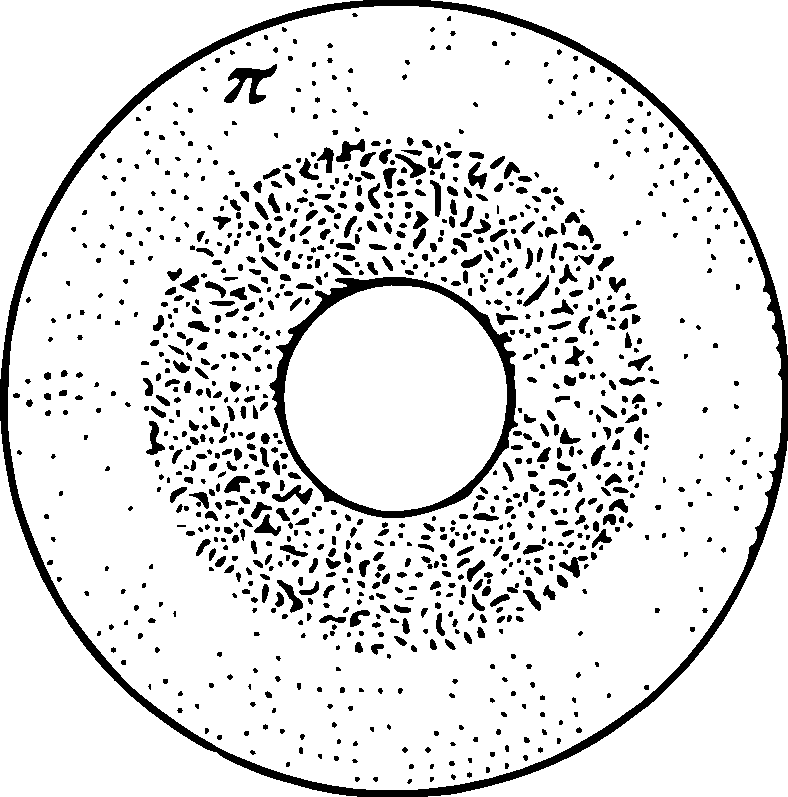
\includegraphics[width=0.8\textwidth]{figs/ch-43/fig-43-04.pdf}
\sidecaption{Schematic visualisation of strcuture of a nucleon.\zhcap{核子结构的示意图。}\label{fig-43-04}}
\end{marginfigure}


\subsection{}\label{43.6.2} The emission and absorption of particles and antiparticles proceed continuously in a nucleon. A nucleon is treated as a complex, incessantly changing assembly of many particles. At the central part of the nucleon (bare nucleon) is the nucleon core having a radius of 0.2 to \SI{0.4d-15}{\meter}. In this region, heavy
particles, resonances and nucleon-antinucleon pairs, play some special role that is not yet quite clear. The outer part of the nucleon forms the pion cloud (\figr{fig-43-04}). This concept of nucleon structure enables the difference in masses of the neutron and proton to be cleared up, as well as the difference of the magnetic moment of the proton and neutron from $\mu_{N}$. These differences are due to energy of electromagnetic interaction between the ``core'' of the nucleon and the pion cloud.
\zhpar{粒子与反粒子在核子内部不断地被发射和吸收。核子被看作由许多粒子组成的、不断变化的复杂集合体。核子的中心部分（裸核子）是核子核心，其半径为 0.2 至 \SI{0.4d-15}{\meter}。在这一区域内，重粒子、共振态以及核子-反核子对扮演着某种特殊的角色，目前这种角色尚不十分清楚。核子的外层形成π介子云（见\figr{fig-43-04}）。这种关于核子结构的概念，可以解释中子与质子质量的差异，以及质子与中子的磁矩相对于 $\mu_{N}$ 的差异。这些差异是由核子的“核心”与π介子云之间的电磁相互作用能引起的。}



\subsection{}\label{43.6.3} The scattering of fast electrons having energies up to \SI{550}{\MeV} by protons enabled the investigation of electric charge density distribution in the proton as a function of the distance $r$ from the centre of the ``core''. It is necessary here to take into account the fact that the charge of the proton is indivisible and is always manifested as a unified whole. Therefore, the  distribution of the electric charge in the proton does not imply the possibility of experimentally separating out a definite part of this charge. 
\zhpar{能量高达 \SI{550}{\MeV} 的快速电子被质子散射，使人们能够研究质子中电荷密度随距离 $r$（距“核心”中心的距离）的分布。在此必须考虑到，质子的电荷是不可分割的，它总是以一个整体的形式表现出来。因此，质子中电荷的分布并不意味着可以通过实验分离出这部分电荷中的某一确定部分。}

\begin{marginfigure}[-2cm] 
\centering
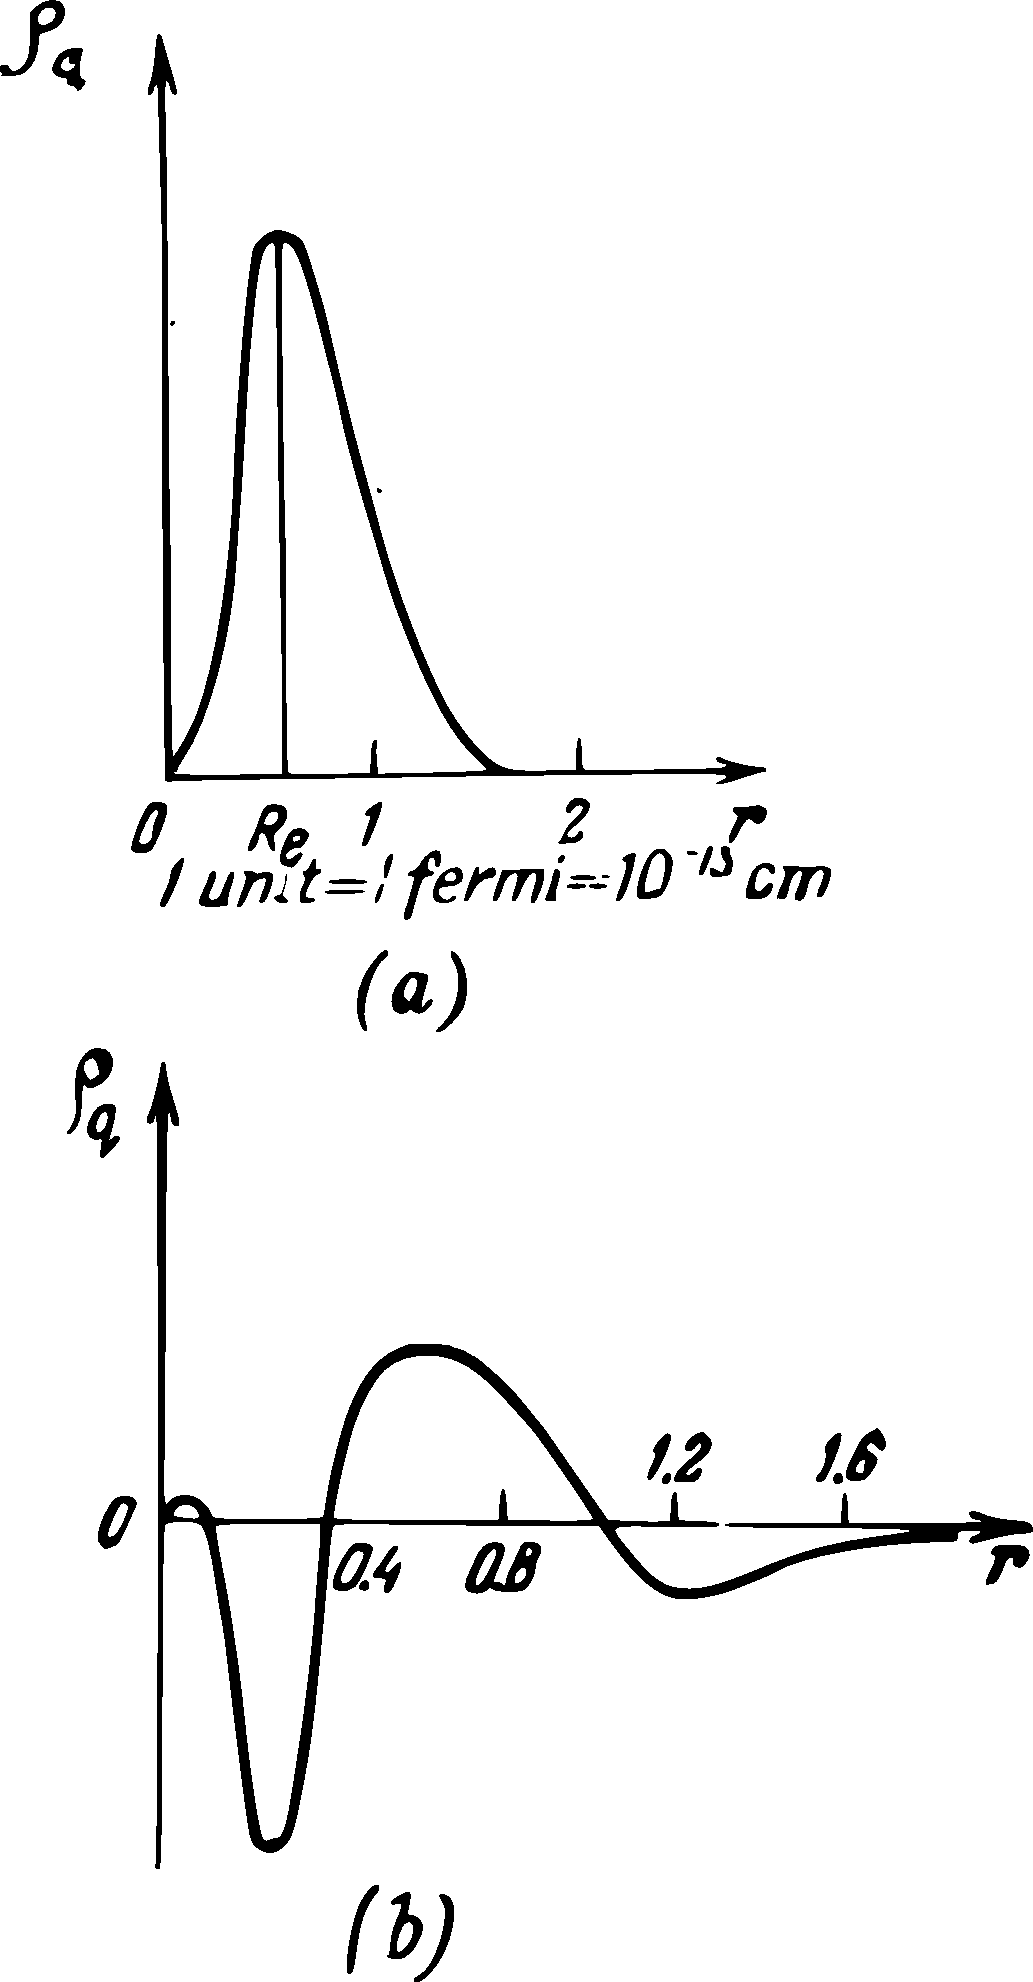
\includegraphics[width=0.8\textwidth]{figs/ch-43/fig-43-05.pdf}
\sidecaption{Schematic visualisation of strcuture of a nucleon.\zhcap{核子结构的示意图。}\label{fig-43-05}}
\end{marginfigure}

Shown in \figr{fig-43-05}~(a) is the dependence of the radial density of charge distribution $\rho_{q} = \dv*{q}{r}$ on $r$ (measured in fermi units), where $\dd q$ is the charge contained in a spherical layer with the radii $r$ and $r + \dd r$. The curve in the figure has a sharply defined maximum at the distance $R_{e} = \SI{0.77d-15}{\meter}$, which is called the ``electric radius'' of the proton. The area under the curve is equal to the charge $e$ of the proton. The results obtained in similar experiments in scattering fast electrons by neutrons are given in \figr{fig-43-05}~(b).
\zhpar{如\figr{fig-43-05}~(a)所示，为电荷径向分布密度 $\rho_{q} = \dv*{q}{r}$ 随 $r$（以费米为单位）的变化曲线，其中 $\dd q$ 为半径分别为 $r$ 与 $r + \dd r$ 的球壳层内所包含的电荷。图中曲线在距离 $R_{e} = \SI{0.77d-15}{\meter}$ 处有一个明显的极大值，该距离称为质子的“电半径”。曲线下的面积等于质子的电荷 $e$。用快速电子对中子进行类似散射实验所得的结果，见\figr{fig-43-05}~(b)。}


Scattering proceeds as if the ``electric radius'' of the neutron was equal to zero. In interaction with fast electrons the neutron behaves as if its pion cloud coincides in dimensions with its ``core''. The electric charge is negative in the inner and outer regions of the neutron; in the middle region it is positive. The total charge of the neutron, equal to the area under the curve, is zero.
\zhpar{散射结果表明，中子的“电半径”等于零。在与快速电子的相互作用中，中子表现得好像其π介子云与其“核心”的尺度相重合。中子的电荷在内部区域和外部区域为负，在中间区域为正。中子的总电荷，即曲线下的面积，等于零。}

The structure of elementary particles is being intensively investigated at the present time.
\zhpar{目前，人们正在对基本粒子的结构进行深入研究。}

% Local Variables:
% TeX-master: "handbook-physics"
% coding: utf-8
% End:
